Our motivating example is Figure \ref{Boulez}, which consists of a small excerpt of music (see \cite[\S 13.1]{Mazzola}, Figure 13.1 for a reference). Our first goal is to realise this as a \emph{global composition} in the formal sense, and then to derive a $\lambda$-term which corresponds to it as a composition. From this example, we hope a general Theory will be formed.
\begin{figure}[h]
 \centering
 \label{Boulez}
 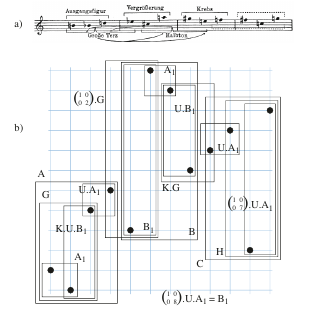
\includegraphics[width = 10cm]{Pictures/Boulez.png}
 \caption{A global composition}
\end{figure}
